\documentclass[10pt,a4paper]{article}
\usepackage[latin1]{inputenc}
\usepackage{amsmath}
\usepackage{amsfonts}
\usepackage{amssymb}
\usepackage{graphicx}

%%% formatting the code
\usepackage{listings}
\usepackage{color}
\lstset{%
	escapeinside={(*}{*)},%
}

\usepackage{hyperref}

\begin{document}

\section{Installing a local AMIDST repository}

Here we explain how to install a local AMIDST repository and how to add
them in a maven project with Java 8 or higher. Alternatively, you can
follow this \href{https://www.youtube.com/watch?v=WvPzJIvGACE}{video
	tutorial}. In summary, we will download the source and use the
appropriate maven commands for installing it.\newline 

First,
you can download the source code from the github repository using the following
command:

\begin{verbatim}
$ git clone https://github.com/amidst/toolbox.git      
\end{verbatim}

Depending on your internet connection, the process may take several minutes. Once the it has finished, enter into the downloaded
folder:\newline 

\begin{verbatim}
$ cd toolbox     
\end{verbatim}

Now, we should install the AMIDST artifact in our local Maven repository (this repository is automatically created when installing Maven). For that, type the following
command:

\begin{verbatim}
$ mvn clean install -Dmaven.test.skip=true   
\end{verbatim}

Note that you can avoid the argument \textbf{-Dmaven.test.skip=true}. In that
case, the process will not skip the unitary tests and hence the
installation process will take much longer (its default value is false).
Once the process has finished, an output similar to the following one
will be generated:\\


\begin{verbatim}
[INFO] Reactor Summary:
[INFO] 
[INFO] AmidstToolbox ...................................... SUCCESS [  0.348 s]
[INFO] core ............................................... SUCCESS [ 12.300 s]
[INFO] core-dynamic ....................................... SUCCESS [  5.352 s]
[INFO] huginlink .......................................... SUCCESS [  3.255 s]
[INFO] standardmodels ..................................... SUCCESS [  3.128 s]
[INFO] examples ........................................... SUCCESS [  4.530 s]
[INFO] moalink ............................................ SUCCESS [  3.944 s]
[INFO] wekalink ........................................... SUCCESS [  2.388 s]
[INFO] ------------------------------------------------------------------------
[INFO] BUILD SUCCESS
[INFO] ------------------------------------------------------------------------
[INFO] Total time: 35.681 s
[INFO] Finished at: 2016-05-10T15:58:14+02:00
[INFO] Final Memory: 63M/539M
[INFO] ------------------------------------------------------------------------
\end{verbatim}

Now we can check that the libraries has been placed into the local maven
repository, which is usually placed in
\textbf{\textasciitilde{}/.m2/repository/}. Thus, type the following
command:\\[3\baselineskip]

\begin{verbatim}
$ ls ~/.m2/repository/eu/amidst/ 
\end{verbatim}

And you will find a folder for each module:

\begin{verbatim}
AmidstToolbox    core-dynamic    huginlink   standardmodels
core        examples    moalink     wekalink
\end{verbatim}

Now we will see how can we use this local repository from a maven
project (using IntelliJ IDEA). In this example, we will use a~ project
containing only one class, though the procedure here explain~ could be
used in any other maven project. You can check this
\href{https://www.jetbrains.com/help/idea/2016.1/getting-started-with-maven.html}{link}
for getting more information about how to create a new mavenproject.\newline 

For using the AMIDST Toolbox, the \textbf{pom.xlm} file will be modified. First,
in the Project view (located on the left) select the file pom.xml of
your project and open it:\newline


\begin{figure}[h!]
\centering	
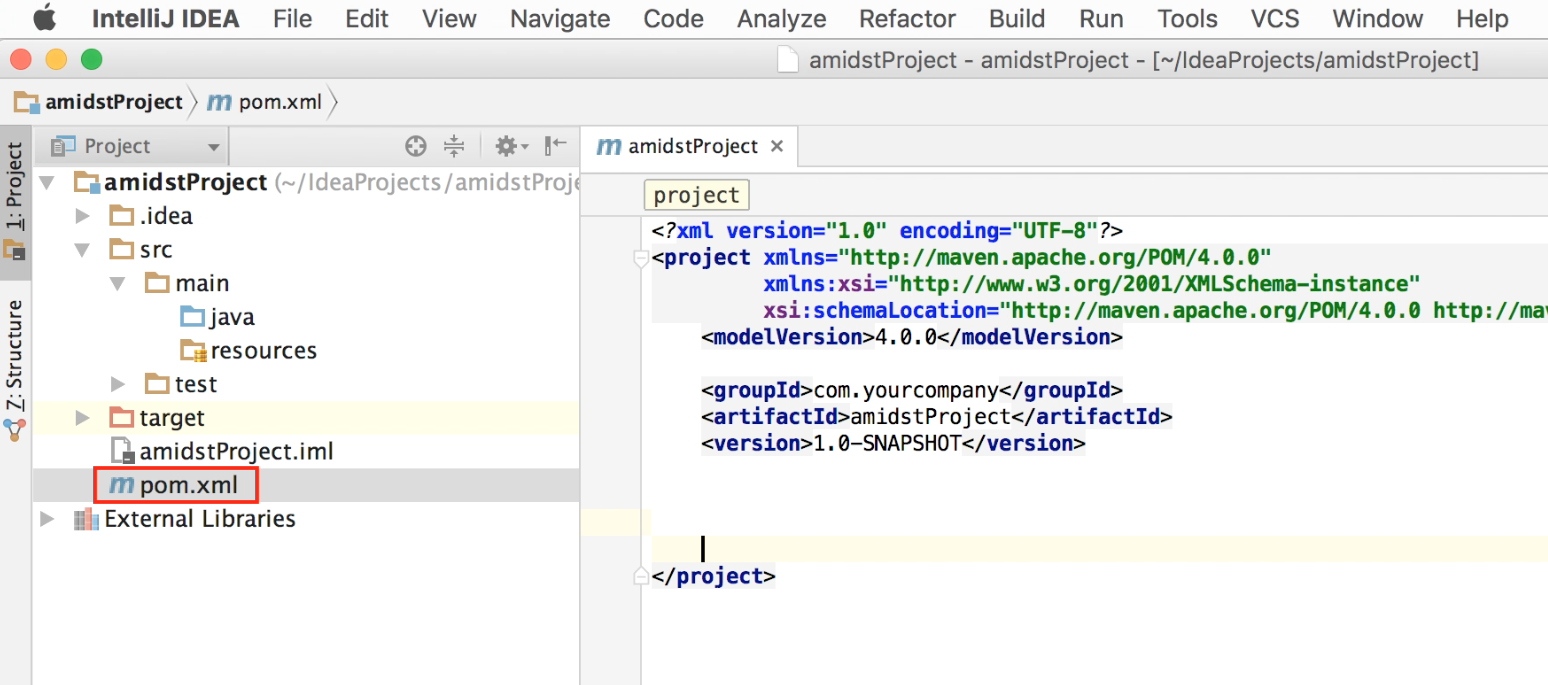
\includegraphics[width=12cm]{img/use_amidst05.png}
\caption{Initial view of an empty maven project in IntelliJ IDEA}
\end{figure}


In the file pom.xml, add the dependencies to the modules in AMIDST you
want to use.~ For each module, add an element
\textbf{\textless{}dependency\textgreater{}\textbf{\ldots{}\textless{}/dependency\textgreater{}}}
inside the labels
\textbf{\textless{}dependencies\textgreater{}\textless{}/dependencies\textgreater{}}.
For each one, we have to indicate the following
information:

\begin{itemize}
	\item
	{groupId} is an identifier of the project's module. In this case it
	should containt the value \emph{``eu.amidst''.}
	\item
	{artifactId }is the name of the module we want to use. More precisely,
	it is the name of the jar file containing such module. You can see the
	list of AMIDST modules
	\href{https://github.com/amidst/toolbox/tree/mvn-repo/eu/amidst}{here}.
	\item
	\textbf{version} is the identifier of~ AMIDST Toolbox release. You can
	see
	\href{mohttps://github.com/amidst/toolbox/blob/master/CHANGELOG.mddules\%20here}{here}
	the list of all versions available.
	\item
	\textbf{scope}~ allows you to only include dependencies appropriate
	for the current stage of the build. We will set this to
	\emph{``compile''.}
\end{itemize}

\noindent For example, for using the {core-dynamic }module, include the
following code:

\begin{verbatim}
<dependencies>
<!-- Load any of the modules from AMIDST Toolbox -->
<dependency>
<groupId>eu.amidst</groupId>
<artifactId>core-dynamic</artifactId>
<version>0.4.2</version>
<scope>compile</scope>
</dependency>

<!-- ... -->
</dependencies>        
\end{verbatim}

Note that for using another module,~ simply change the value of the
element artifactId{ }(i.e. the content between the tags
\textless{}artifactId\textgreater{} and
\textless{}artifactId\textgreater{}). Now you can check in the \textbf{Maven Projects panel} that all the
dependencies have been loaded:


\begin{figure}[h!]
	\centering	
	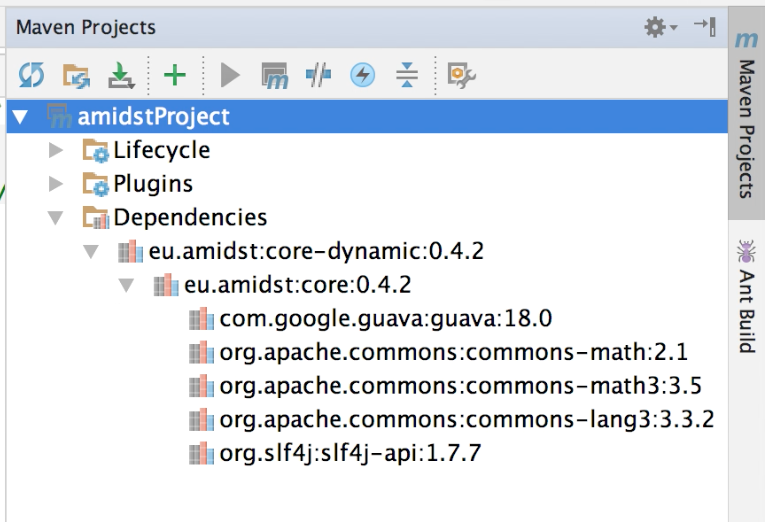
\includegraphics[width=12cm]{img/use_amidst07.png}
	\caption{Loaded dependencies}
\end{figure}



Note that the \emph{core-dynamic module} depends on {core }{}that has
been loaded as well. We recomend you to download the sources and the
javadoc as shown below.


\begin{figure}[h!]
	\centering	
	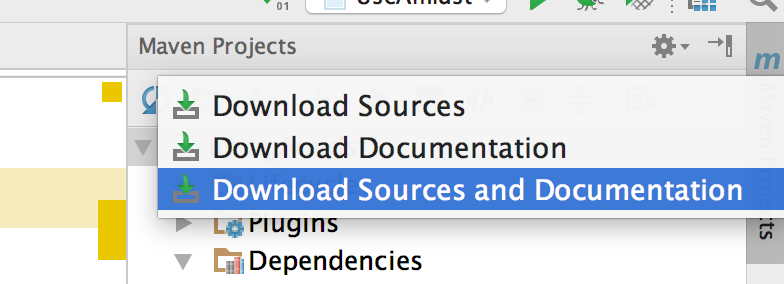
\includegraphics[width=12cm]{img/use_amidst08.png}
	\caption{Downloading JavaDoc and source code}
\end{figure}

\newpage 


\noindent Finally, for testing purposes, we can run the following
code:\newline 

\begin{verbatim}
import eu.amidst.dynamic.models.DynamicBayesianNetwork;
import eu.amidst.dynamic.utils.DynamicBayesianNetworkGenerator;

public class TestingAmidst {
 public static void main(String[] args) throws WrongConfigurationException {
  DynamicBayesianNetworkGenerator.setNumberOfContinuousVars(2);
  DynamicBayesianNetworkGenerator.setNumberOfDiscreteVars(5);
  DynamicBayesianNetworkGenerator.setNumberOfStates(3);

  DynamicBayesianNetwork extendedDBN = 
  DynamicBayesianNetworkGenerator.generateDynamicBayesianNetwork();

  System.out.println(extendedDBN.toString());


 }

}
\end{verbatim}

\noindent If everything goes right, the following output will be
generated:\newline 


\begin{figure}[h!]
	\centering	
	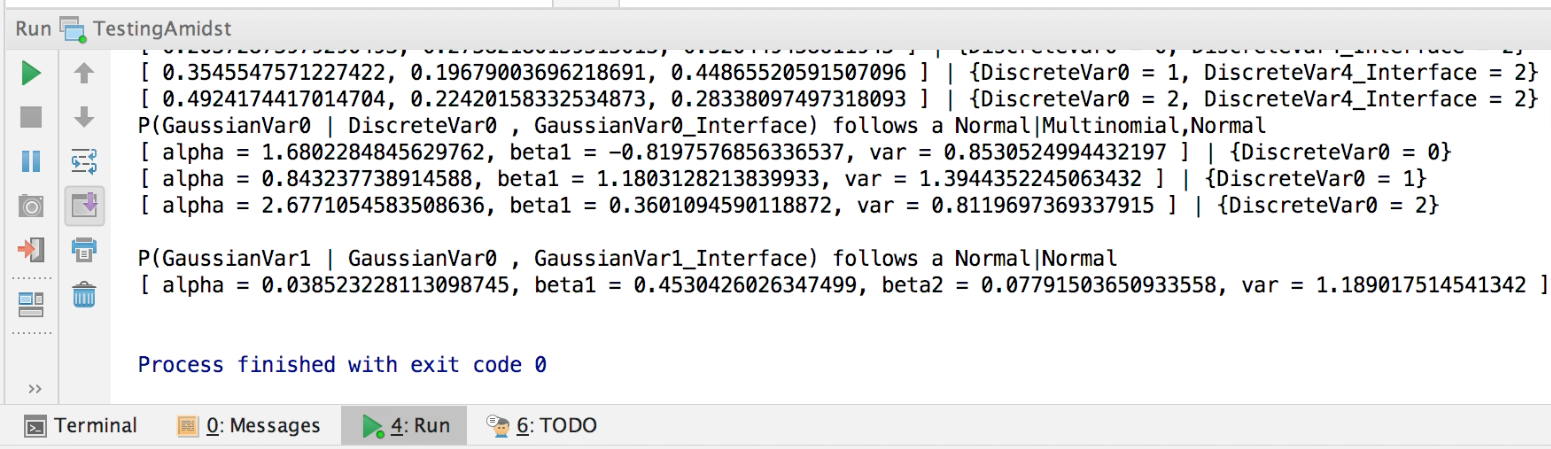
\includegraphics[width=12cm]{img/use_amidst09.png}
	\caption{Output generated when running the example code}
\end{figure}
\end{document}